\section{Senzor teploty}
\label{sec:perif-sensor-teploty}
    Cílem tohoto modulu je kontinuálně měřit teplotu vody a naměřená data poskytovat řídicí jednotce skrze sběrnici \acs{can}. Při volbě konkrétního teplotního čidla je potřeba vzít v potaz několik faktorů:
    \begin{itemize}
        \item Přesnost a rozsah
        \item Časová stálost
        \item Složitost implementace 
        \item Pouzdro určené pro ponoření do vody
        \item Cena
    \end{itemize}

    \subsection{Metody měření teploty}
        Nejčastěji používanými součástkami určenými k měření teploty jsou nepochybně termistory a termočlánky~\cite{allaboutcircuits2023tempsensors}. Termistor je rezistor vytvořen z materiálu, který mění svůj odpor v závislosti na teplotě přičemž rozlišujeme dva základní typy termistorů podle toho, zda s rostoucí teplotou jejich odpor roste (PTC termistor) anebo klesá (NTC termistor). U obou typů lze obecně říci, že závislost odporu na teplotě je značně nelineární, pro zjištění přesné teploty je tedy potřeba buďto měřená data dále zpracovat (např. mikrokontrolérem) anebo využít speciální integrovaný obvod, který výstup z připojeného termistoru linearizuje a dále propaguje buďto v analogové nebo i digitální podobě. Jelikož odpor termistoru a stejně tak i dalších součástek, potřebných k jeho zapojení, má jistou výrobní toleranci, je vhodné sensor před použitím kalibrovat.

        Princip termočlánku je odlišný, jedná se o vodivé spojení dvou kovů na kterém díky Seebeckově jevu vzniká termoelektrické napětí. Velikost tohoto napětí je daná použitými materiály a je také teplotně závislá. V praxi se používá nejčastěji několik dvojic materiálů, které svými vlastnostmi a cenou nejvíce vyhovují běžným požadavkům, ty pak získaly také své označení jako termočlánky typu J, K, T nebo E (typů existuje více, uvedeny jsou nejčastěji používané~\cite{TechieScience_Thermocouples}). Termočlánky pracují oproti ostatním senzorům s výrazně větším rozsahem teplot a mohou měřit také teploty velmi vysoké. Nevýhodou je nízké výstupní napětí, které musí být spolehlivě měřeno, tedy ideálně porovnáno s přesnou napěťovou referencí a také je potřeba, aby část zařízení, ke kterému je termočlánek připojen (tzv. studený konec), byla udržována při konstantní referenční teplotě anebo případnou změnu teploty měřila jiným způsobem a kompenzovala výpočtem~\cite{allaboutcircuits2023tempsensors,TechieScience_Thermocouples}.

        Z hlediska praxe je další často využívanou možností použití zcela integrovaného sensoru s digitálním výstupem. Pro zpracování je sice potřeba mikrokontrolér, ale tyto sensory bývají od výroby kalibrovány a také jejich zapojení je velmi jednoduché, což je výhodou.

    \subsection{Realizace sensoru}
        Při porovnání uvedených metod se použití termočlánku jeví jako nevhodné, zejména kvůli náročnosti implementace, která současně navyšuje také cenu. Zbývá tedy rozhodnutí mezi termistorem a digitálním čidlem. Ve voděodolném pouzdře lze zakoupit jak několik variant termistorů, tak i digitální čidlo (zde DS18B20). Nejlevněji vychází termistor typu NTC, ale v porovnání s cenou celého zařízení je rozdíl v ceně zanedbatelný.     
        
        \begin{figure}[!ht]
            \centering
            \begin{circuitikz}
                \ctikzset{resistor = european}
                % Draw the DS18B20 sensor
                \draw (0,0) node[rectangle, draw, minimum width=3cm, minimum height=4cm] (ds18b20) {};
                \node[anchor=north] at (ds18b20.south) {DS18B20};
                
                % Draw the pins on the DS18B20
                \draw (ds18b20.north east) ++(0,-0.5) coordinate (pin1);
                \draw (ds18b20.north east) ++(0,-2.5) coordinate (pin2);
                \draw (ds18b20.north east) ++(0,-3.5) coordinate (pin3);
                \node[left] at (pin1) {VDD};
                \node[left] at (pin2) {DATA};
                \node[left] at (pin3) {GND};
                
                % Draw the \acs{mcu}
                \draw (7,0) node[rectangle, draw, minimum width=3cm, minimum height=4cm] (mcu) {};
                \node[anchor=north] at (mcu.south) {PIC18F26};
                
                % Draw the pins on the \acs{mcu}
                \draw (mcu.north west) ++(0,-0.5) coordinate (mcupin1);
                \draw (mcu.north west) ++(0,-2.5) coordinate (mcupin2);
                \draw (mcu.north west) ++(0,-3.5) coordinate (mcupin3);
                \node[right] at (mcupin1) {VDD};
                \node[right] at (mcupin2) {RC7};
                \node[right] at (mcupin3) {GND};
                
                % Connect DS18B20 to \acs{mcu}
                \draw (pin1) -- (mcupin1);
                \draw (pin2) -- (mcupin2);
                \draw (pin3) -- (mcupin3);
                
                % Add pull-up resistor
                \draw (mcupin1) ++(-1,0) to[R, l_=4.7k, *-*] ++(0,-2);
                
            \end{circuitikz}
            \caption{Připojení čidla DS18B20 k \acs{mcu}.}
            \label{fig:temp-sensor-pripojeni}
        \end{figure}

        Pro realizaci sensoru bylo zvoleno digitální čidlo DS18B20, které narozdíl od termistoru není potřeba kalibrovat a výrobce garantuje přesnost \(\pm \qty{0.5}{\degreeCelsius}\) na celém teplotním rozsahu od \qty{-55}{\degreeCelsius} do \qty{+125}{\degreeCelsius}. Rozlišení sensoru je až 12 bitů, tedy minimální měřitelná změna teploty odpovídá \qty{0.0625}{\degreeCelsius}. Pro komunikace s čidlem se využívá protokol 1-Wire, kdy datový vodič funguje obousměrně, pro propojení čidla s mikrokontrolérem tedy stačí využít tři vodiče a jeden pull-up rezistor, viz obr.~\ref{fig:temp-sensor-pripojeni}. 

        \begin{figure}[h!]
            \centering
            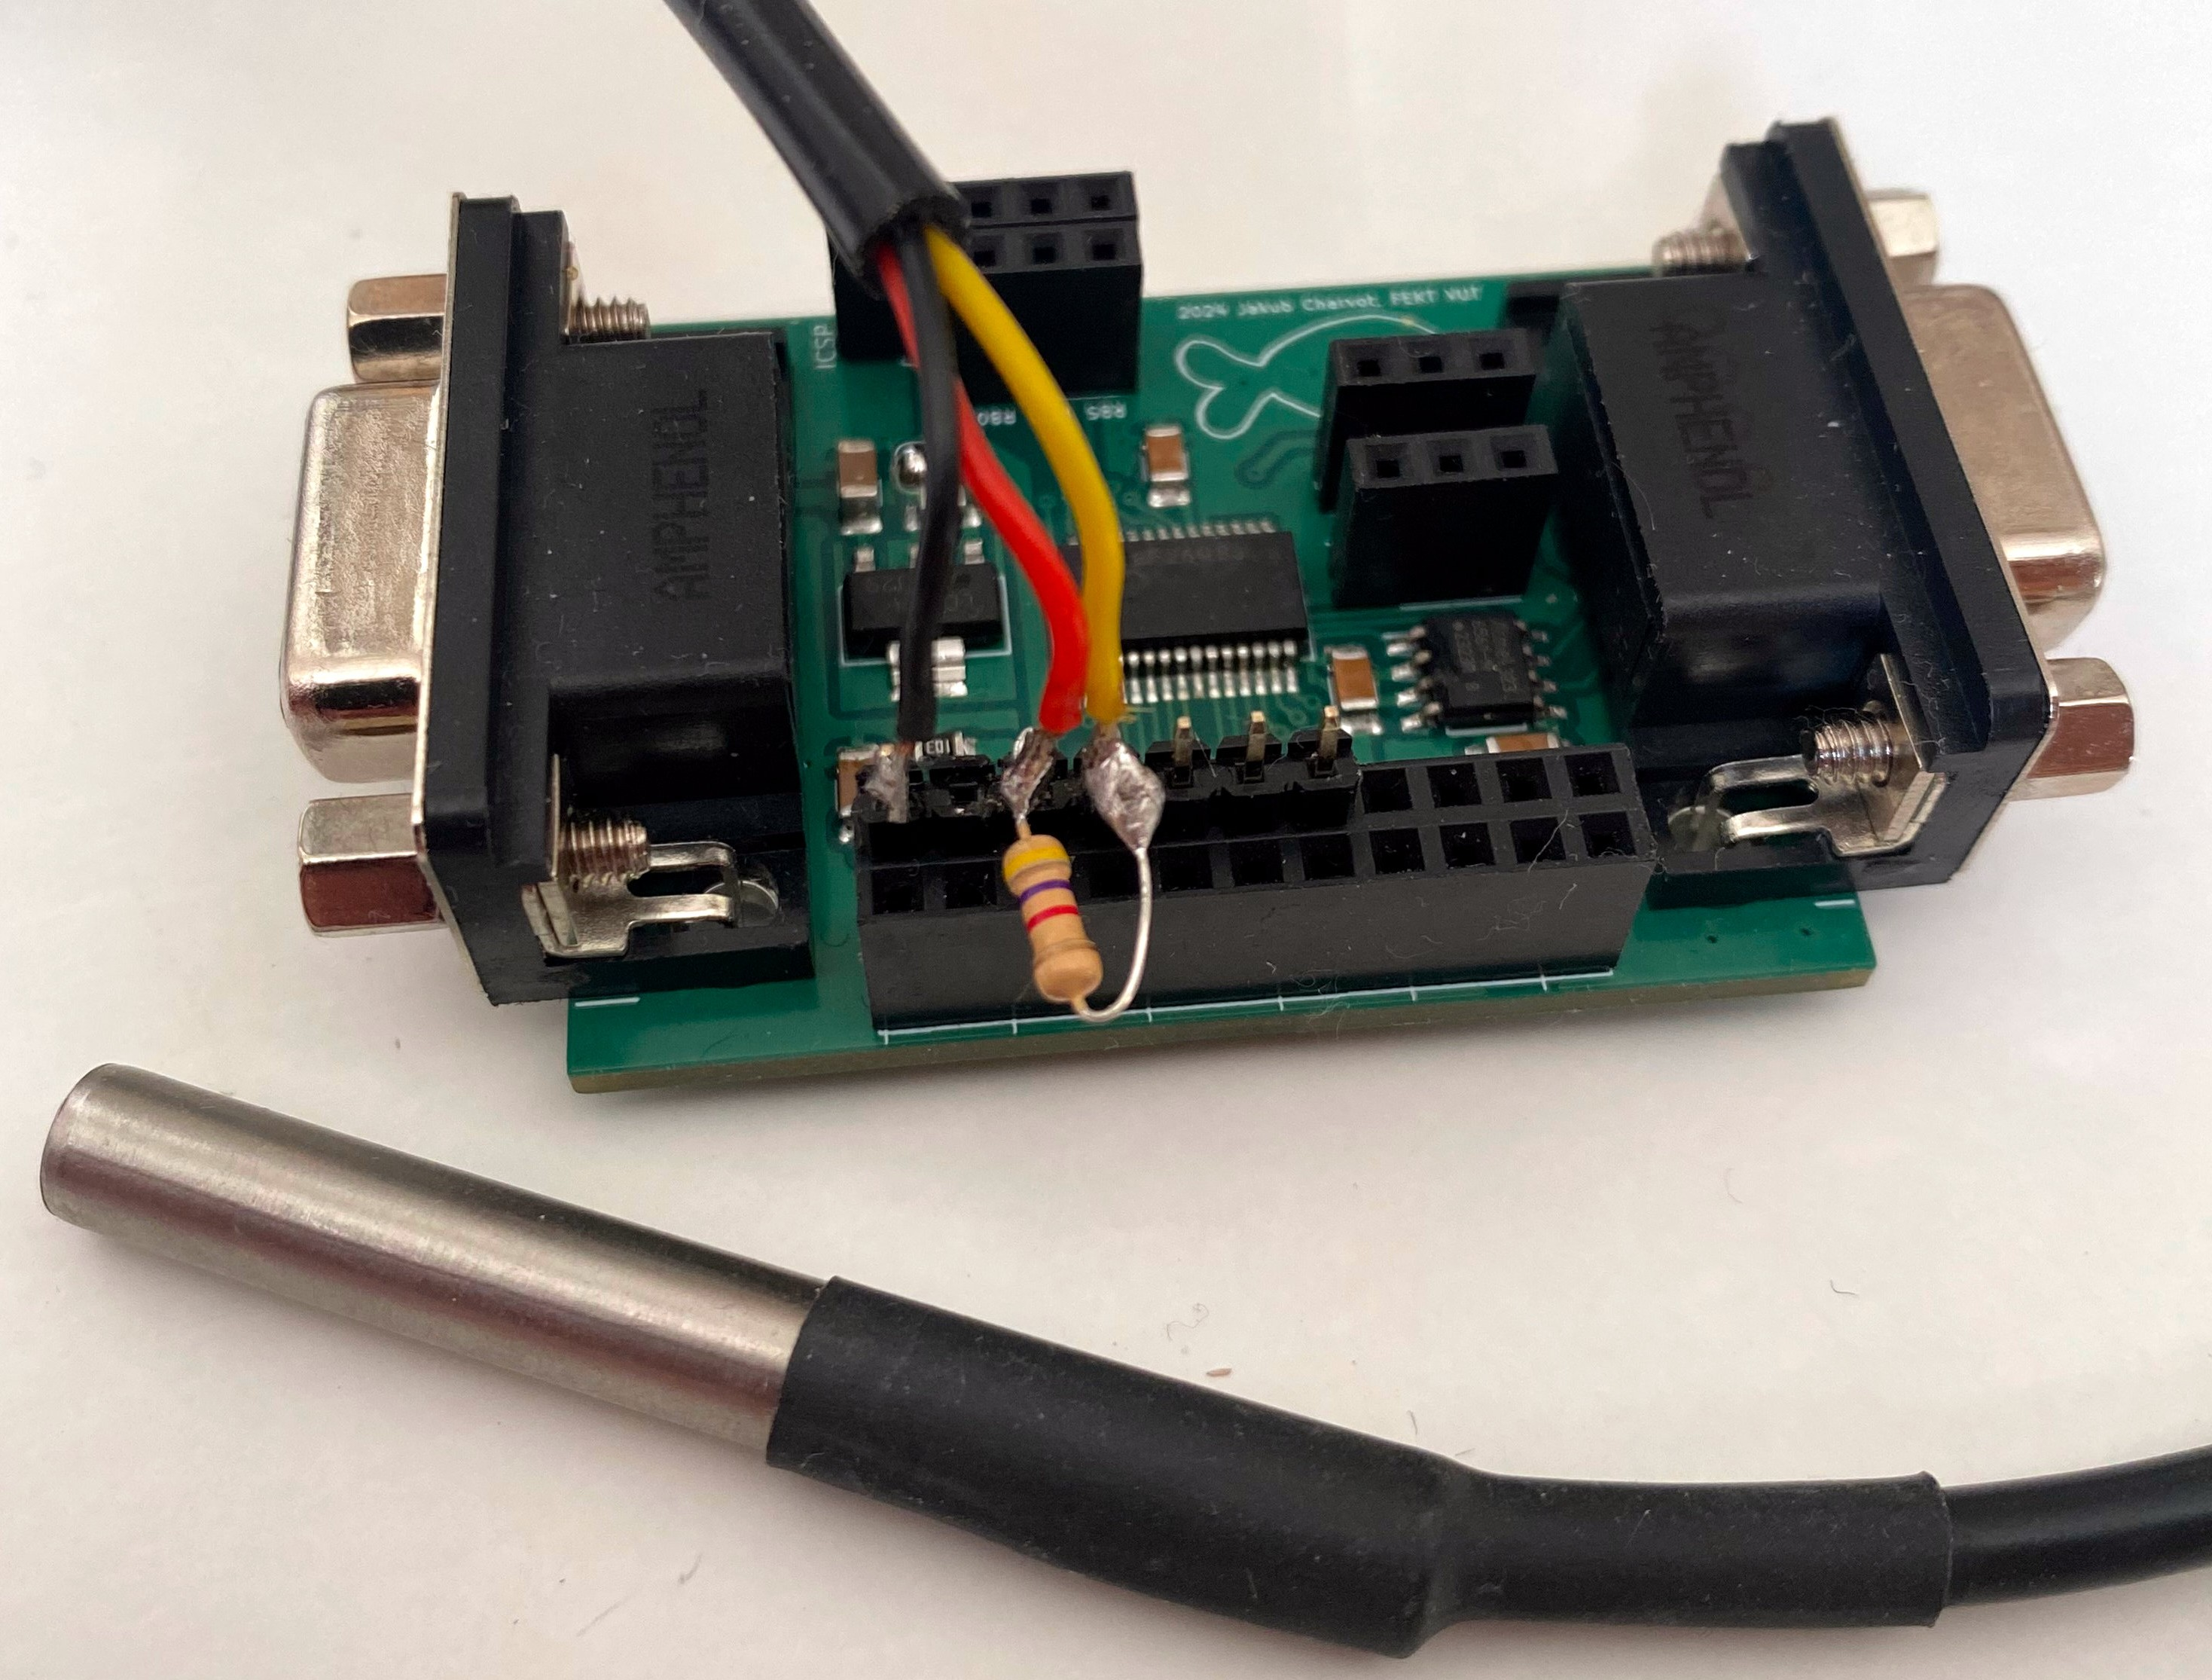
\includegraphics[width=0.8\textwidth]{obrazky/foto/sensor_teploty.jpeg}
            \caption{Realizovaný sensor teploty s čidlem DS18B20.}
            \label{fig:obrazky-foto-sensor_teploty}
        \end{figure}
        
        
        Fyzické připojení čidla k obecnému module periferie bylo provedeno za pomocí jedné pinové lišty, ke které jsou připájeny vývody čidla a stejně tak i pull-up rezistor. Výsledná podoba realizovaného senzoru je vidět na obr.~\ref{fig:obrazky-foto-sensor_teploty}. V budoucnu bude modul vsazen ještě do vlastní krabičky.